\documentclass[conference]{IEEEtran}
\IEEEoverridecommandlockouts
% The preceding line is only needed to identify funding in the first footnote. If that is unneeded, please comment it out.
\usepackage{cite}
\usepackage{amsmath,amssymb,amsfonts}
% \usepackage{algorithmic}
\usepackage{graphicx}
\usepackage{float}
\usepackage{textcomp}
\usepackage{xcolor}
\usepackage{booktabs}
\usepackage{algorithmicx}
\usepackage{algpseudocode}
\usepackage[ruled,vlined,linesnumbered]{algorithm2e}
\usepackage{subcaption}
\captionsetup{compatibility=false}
\usepackage{multirow}
\def\BibTeX{{\rm B\kern-.05em{\sc i\kern-.025em b}\kern-.08em
    T\kern-.1667em\lower.7ex\hbox{E}\kern-.125emX}}
\begin{document}

\title{A Distributed Bilateral Resource Market Mechanism for Future Telecommunications Networks}
% {\footnotesize \textsuperscript{*}Note: Sub-titles are not captured in Xplore and
% should not be used}
% \thanks{Financial support from Science Foundation Ireland grants 14/IA/252 (O'SHARE) and 13/RC/2077 is gratefully acknowledged. This material is based upon work supported by Google Cloud.}
\author{\IEEEauthorblockN{Nima Afraz and Marco Ruffini}
\IEEEauthorblockA{\textit{CONNECT CENTRE} \\
\textit{The University of Dublin, Trinity College, Ireland}\\
% City, Country \\
\{$nafraz, marco.ruffini\}$@tcd.ie}}


\maketitle

\begin{abstract}
In this paper, we propose a distributed market mechanism powered by the blockchain technology addressing network ownership models in multiple telecommunications networks use cases. The proposed model is based on the smart contract technology and enables transparent and trusted bilateral trades, where trust among the network operators does not exist, and there is no impartial third-party entity who is trusted by all of the participants. We use an open source permissioned blockchain framework called Hyperledger Fabric to investigate the performance of the distributed market mechanism in cloud environments. After running experiments on Hyperledger Fabric, we discuss the practical feasibility and possible design choices of our blockchain approach based on latency, throughput and resource consumption analysis.

%can help with the feasibility analysis of the blockchain application and making design choices.
\end{abstract}

\begin{IEEEkeywords}
Blockchain, Market, Double auction, Smart Contract, telecommunications operators, virtual network operators.
\end{IEEEkeywords}

\section{Introduction}

% Concentration of network infrastructure ownership in current telecommunications sector will negatively contribute to the widespread deployment of the fifth generation (5G) mobile networks as the their decision will be entangled to the potential revenue generating opportunities. However, most of the current applications for 5G networks might not be considered commercially fruitful enough for the operators to justify such a massive investment to deploy new 5G networks.  
Widespread deployment of the fifth generation (5G) networks will require the ability of the network infrastructure providers (IP) to assure new revenue streams in order to compensate the capital expenditure incurred with the new network. New services will require novel business models as they are unlikely to fit within current network ownership models, where an Over-The-Top service provider (OTT) or a vertical industry has to undergo manual negotiations to acquire a unit of the network resources to deliver services to its customers. Therefore, automated business processes become vital as they can facilitate the utilization of the network infrastructure for new services, as they appear.


Blockchain technology has already been adopted by a wide range of industries to automatize complex business processes and workflows \cite{fridgen2018cross,milani2016blockchain}. Blockchain technology helps these enterprises to move away from the Business Process Management (BPM) models where a third party organization stores the business information in a central repository and controls the transactions in cross-industry environments. This way, they both avoid the single point of failure and allow enterprises to gain control of their own data.


The business process we are interested in automating is the process of dedicating a set of network resources to a Virtual Network Operator (VNO) on-demand, for a given period of time. Furthermore, giving the ability to the VNO to trade their excess resources with others. In particular, we are interested in studying the implementation of bilateral resource trading markets using blockchain as the data storage structure solution and smart contracts as the tool for the execution of the market mechanisms and inter-carrier financial settlement. The examples of such bilateral trade markets in telecommunications industry include: resource allocation in Network Function Virtualization (NFV) markets \cite{8542782}, promoting femtocell access \cite{8665886}, mobile crowd sensing with budget constraint \cite{8664672}, spectrum allocation \cite{8395445} and multi-tenant Passive Optical Networks (PONs) \cite{8488596}. The common challenge among these resource markets is the fact that they rely on a third-party broker to both store the private financial information of the participants and execute the auction mechanisms which directly determine the allocation of the resources.

In this paper, we examine how blockchain technology can enable the automation of a business process, i.e., bilateral trade of network resources in an inter-carrier business environment with no mutual trust among the participants.

We first describe the manual cycle of these business processes and the challenges associated with it. Then, we model the bilateral trade of network resources in the context of smart contracts and blockchain transactions. Finally, we report and discuss the results of our experiments using Hyperledger Fabric \cite{Fabric}, a permissioned blockchain framework.


\section{Distributed Resource Market Model}
Network sharing lowers the cost of network roll-out by preventing the costly duplication of network infrastructure. The traditional roles of an infrastructure provider and VNOs are being challenged with new market players such as OTTs and vertical market services (e.g., automotive, e-health, etc.) which are considered to be the major revenue generation sources for future 5G networks.
These are typically scenarios where network investment and 5G deployment would be very costly or unattractive for legacy operators, but verticals expect instead significant advantage (i.e. there is a large private value for specific applications that require 5G type of connectivity).

Moving from conventional static sharing towards on-demand/on-the-fly dynamic multi-tenancy \cite{7514161} requires a network sharing management architecture that enables capacity brokering.

To understand the importance of automating such bilateral market business processes it is necessary to know how the current process works.
A bilateral trade market is a business environment where multiple traders in both seller and buyer roles can exchange commodities (e.g., network resources). Furthermore, in this work, we will allow the traders to change their role in the market (i.e., seller or buyer) depending on their current excess/demand of resources.
A typical bilateral market trade can involve: 
\begin{itemize}
    \item The manual negotiation of the terms of trade between the VNOs. This includes the price setting, which if happens manually, will not allow dynamic high-frequency trading of the resources.
    \item Different interpretations of the negotiated terms. In such a case, a third-party authority (e.g., regulator, infrastructure provider, etc.) could be summoned to solve the dispute; however, this implies additional delays and cost for the VNOs.
    \item Lack of trust among the VNOs and absence of a trusted central authority holding the market by enforcing the terms. 
\end{itemize}

These issues mean that VNOs have little incentive to participate in a dynamic resource trading market.


Many resource/infrastructure sharing problems in the communications sector are modelled as bilateral trade markets as these markets are capable of supporting multiple participants on both sides of the market. The majority rely on solutions based on game theory, in order to match supply and demand \cite{8542782,8665886,8664672,8395445,8488596}. One of the most prominent solutions is the double auction, which focuses on allocating commodities (i.e., resources) to the participants with the highest demand. The end goal is to achieve the highest Social Welfare (i.e., maximizing the aggregate of all participants' utilities) in the market. 

In this paper, we use an implementation of the double auction, which was originally designed for resource sharing in multi-tenant passive optical networks (details of the auction mechanism can be found in \cite{8488596}). The auction mechanism is capable of providing an allocation scheme for the resources while assuring ''Truthfulness'' among the participants (i.e., providing positive incentives to avoid manipulative market behaviour). However, in our previous work, we made the assumption that this market model depends solely on a central third-party authority (the infrastructure provider), which is trusted by all of the market participants. This central authority is thus in charge of both record-keeping of the market data and conducting the auction on behalf of all participants. 

Considering however that it is quite typical for an infrastructure provider that shares its network to also offer services, in competition with other VNOs, it is unrealistic to assume that VNOs will trust the infrastructure provider. Being in competition with other VNOs, the infrastructure provider could benefit from manipulating the market data or the process of the auction mechanism. 

Therefore, we propose a new distributed model for bilateral trade markets, which eliminates the reliance on an impartial central authority. This is achieved making use of the two following features of blockchain:

\begin{itemize}
    \item Distributed record keeping of all the transactions and participants data using the distributed ledger technology.
    \item Conducting the auction in a distributed fashion rather than centralized, enabled by the smart contract technology.
\end{itemize}



The transaction flow is illustrated in Fig.  \ref{fig:flow}. The application sends the transaction proposal to the orderer, to be broadcast to the peers in the channel. A transaction in the context of this paper is the process of receiving the bids/asks from the traders and conducting the double auction, matching eligible sellers and buyers and issuing the results of the resource allocation. The peers proceed with the endorsement of the transactions (i.e., the auction) based on the predefined endorsement policy. The endorsed transaction is then returned to the application and sent to the orderer to finalize the ordering of the transactions into a block (using one of the consensus protocols available, e.g., Solo, Kafka, Raft).

\begin{figure}
    \centering
    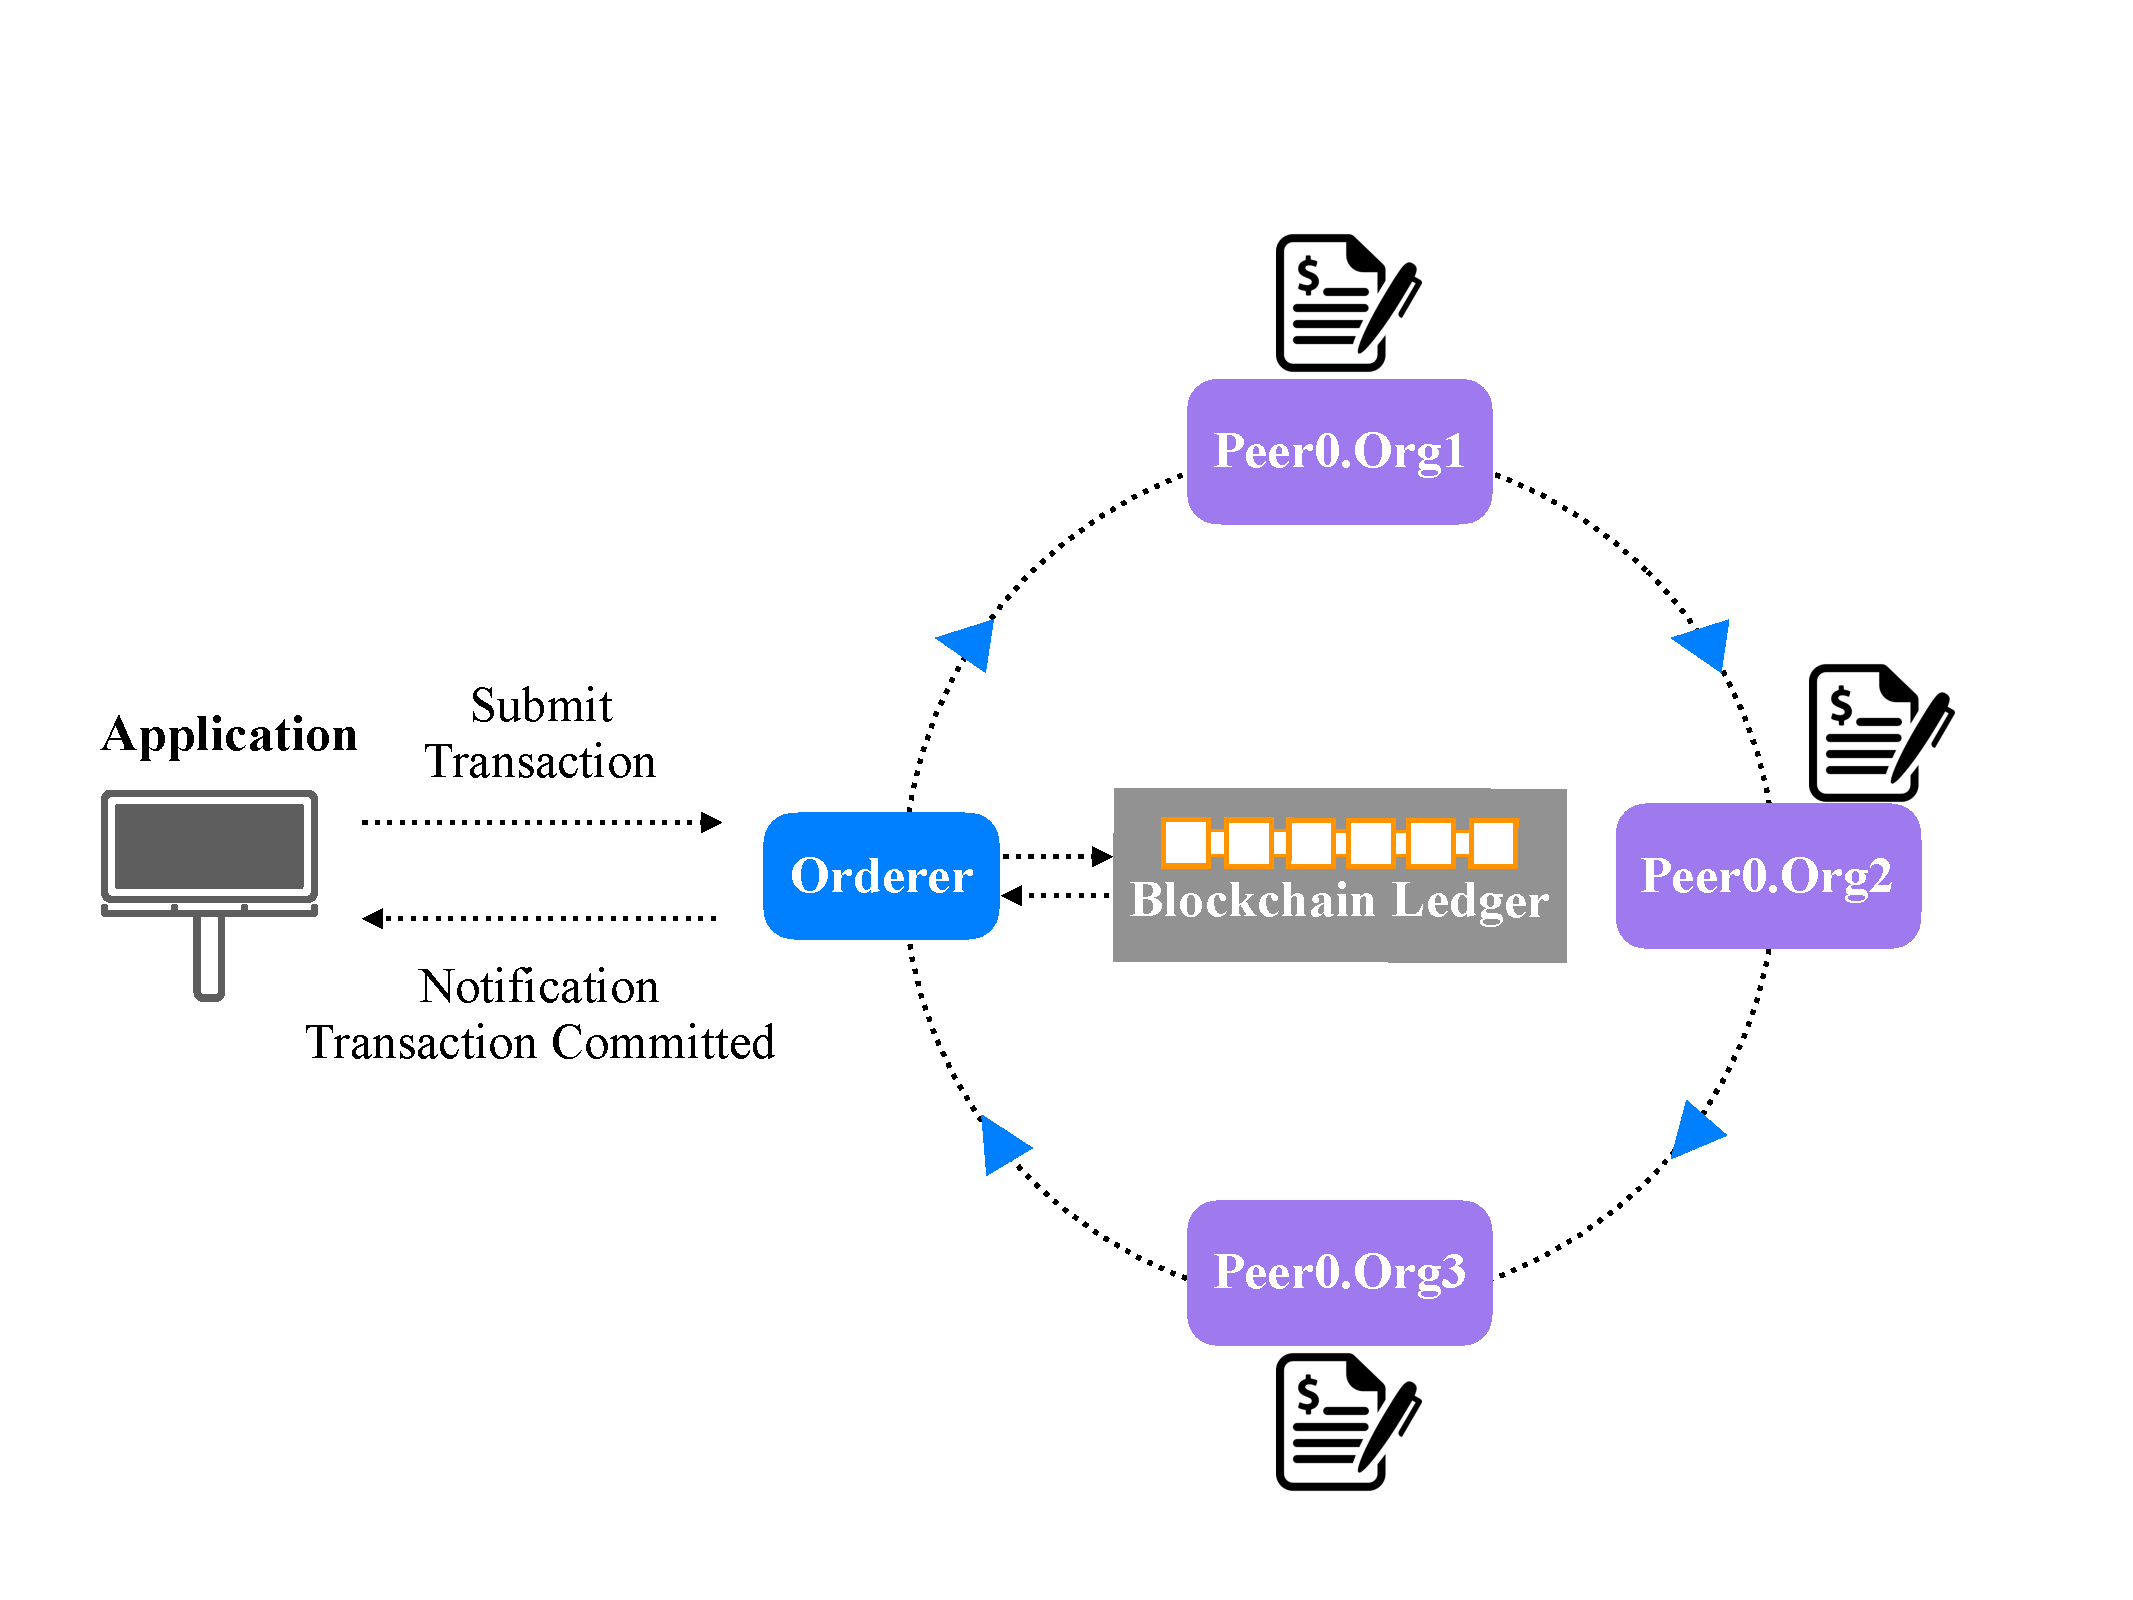
\includegraphics[width=0.49\textwidth]{figs/Fig.pdf}
    \caption{The blockchain transaction flow}
    \label{fig:flow}
\end{figure}

\section{Application of Blockchain to private markets}
Blockchain is a tool that provides a novel record-keeping method that is distributed, transparent, immutable, and anonymous. As a concept, blockchain challenges the blind trust on the numerous central authorities who are currently in charge of vital and critical transactions among users and enterprises. 
Bitcoin, the most well-known use case for blockchain technology, has been known as the front face of the technology. Bitcoin is a digital asset or a cryptographic currency designed to remove the dependency on a central authority (a bank in this case) to achieve trust among its users.
The main innovation of  Blockchain is preventing double-spending while offering a distributed alternative to the costly real-world central bank system, which provides the required mechanisms to avoid double-spending. In short, blockchain technology provides a robust solution for trustable bookkeeping.


Blockchain technology is being considered as the primary trust solution when a trustworthy central bookkeeper is absent. Example applications are Government and Private Management, Electronic Voting, Authorship and Ownership, etc. \cite{8552978}, while more are currently under study, such as applications in pharmaceutical supply-chain \cite{7987376}, Consumer Electronics \cite{8386955}, smart-cities \cite{8386958}, privacy protection in health-care \cite{8386918} and insurance \cite{8386868}. % It was later realized that the cryptocurrency application does not fully utilize the potential of blockchain technology. In other words, the same decentralized consensus mechanism could be used to maintain the same level of trust for the logic-enabled transaction rather than simple bookkeeping. 

%The idea of blockchain was further complemented by the concept of smart contracts which introduced the blockchain technology, not only as a robust bookkeeping tool but also as an effective automation platform which can address many trust-related concerns in multi-party business ecosystems. A Smart Contract is an immutable piece of logic (computer program) that enhances the distributed ledger technology with self-enforcing pre-negotiated agreements.

In this paper, we target the blockchain's features that enables automating the inter-operator agreement and settlement processes. For instance, in \cite{8368442} the authors propose a decentralized power market framework based on blockchain and smart contract that can offer independent maintenance and management of the transactions along with the automatic transfer of funds between the market players.

On the other hand, adopting blockchain for business to business ecosystems raises concerns about the access control to the sensitive business data written on the ledger. The primary blockchain technologies address this issue by providing a pseudo-anonymous environment where the owner of the digital assets can be kept private. However, businesses would require additional levels of authentication to assure the security of the transaction and financial data. 
This cannot be guaranteed by permissionless blockchains (i.e., the type used by bitcoin), where contributing to the validation of the transactions and creating the blocks does not require any form of permission or authorization.
%Blockchains such as Bitcoin are referred to as permissionless blockchains, i.e., where contributing to the validation of the transactions and creating the blocks does not require any form of permission or authorization. This feature makes the blockchain technology more interesting for business use-cases as the identities of the participants are known; therefore, they can be held accountable and also the ledger data is not publicly available over the network.

The Hyperledger project was thus initiated to provide a solution for some of the issues raised by permissionless blockchains. Hyperledger is an open source project hosted by the Linux Foundation with the purpose of providing blockchain technologies for businesses. Numerous purpose-specific frameworks and tools are being developed under the Hyperledger's umbrella for the use-cases ranging from finance and banking to the Internet of things, supply chain management and manufacturing.
Hyperledger Fabric is one of the frameworks which provides a permissioned distributed ledger technology for cross-industry applications, i.e. where only specific entities are allowed to participate. The main features of the Hyperledger Fabric platform are as follows:

\begin{itemize}
    \item It is a modular architecture which allows plug-and-play implementations of different functions/components such as consensus, membership service, etc.
    \item It uses open source container technologies (i.e., Docker) to host different components of the blockchain network
    \item It makes use of permissioned membership management and access to the ledger
    \item It allows for chaincode (smart contracts) to be written in various programming languages (e.g., Go, JavaScript, or Java) while other blockchain platforms only allow specific languages (e.g., Solidity in Ethereum)
    
\end{itemize}

A Fabric network consists of multiple components including the following:

\begin{itemize}
    \item Ledger(s): immutable data storage tool that keeps the records of the transactions. A Fabric network might contain multiple ledgers.
    \item Organizations: the blockchain network consists of one or multiple organizations who are contributing resources to the network while being able to process their transactions with other participants. Organizations host peers and other components of the network and each maintains a copy of the ledger.
    \item Peers: Hosted in Docker containers with different roles including endorser, versifier etc.
    \item Orderer(s): The component responsible for ordering the transactions into blocks to be written on the blockchain.
    \item Chaincode (Smart contract): A piece of computer program which sits on the blockchain and works in a self-enforcing fashion.
    \item Channels(s): A feature of the Fabric which allows data isolation among different organizations/participants in the network, in order to ensure privacy.
\end{itemize}

% consists of different types of entities, peer nodes, ordering service nodes and clients, belonging to various organizations. Each of these has an identity on the network which is provided by a Membership Service Provider (MSP) [9], typically associated with an organization. All entities in the network have visibility to the identities of all organizations and can verify them.





\subsection{Performance Criteria}
A blockchain application operates over an underlying network of different components. The performance of the application is closely tied to the performance of each component (e.g., peers, orderers, containers, etc.) and the network that interconnects them. The performance of a blockchain application/network can be measured using the following metrics:

\begin{itemize}
    \item Transaction Throughput, measured in transactions per second (TPS):
    The number of transactions that are processed by the blockchain and written on the ledger in a given second.
    
    \begin{equation} \label{eq1}
    \begin{split}
    Transaction\,Throughput = \frac{Total\,Transactions}{Total\,time\,in\,seconds}
    \end{split}
    \end{equation}

    \item Transaction Latency:
    The amount of time taken from the moment when a transaction is submitted until the moment when it is confirmed and available on the blockchain. This includes the propagation time and the processing time due to the consensus/ordering mechanism.
    
    \begin{equation} \label{eq2}
    \begin{split}
    Transaction\,Latency = t_{Confirmation} - t_{Submission}
    \end{split}
    \end{equation}



    \item Computing Intensity:
    The amount of computing resources consumed by the blockchain throughout the operating time, including the processing power, memory, storage, I/O and network. This metric is of great importance as it could determine the cost efficiency of a blockchain application. Furthermore, besides the capital expenditure for providing the computing capacity, blockchain networks could require huge amounts of energy to operate. Therefore, the computing intensity would also affect the operation costs of the blockchain.
    

\end{itemize}

In the next section, we introduce a benchmark tool that enables the measurement of the above mentioned performance metrics in various blockchain platforms. We also report on the results of our experiments with implementing the bilateral resource market on a Hyperledger Fabric framework.



\begin{figure*}
% \vspace{-7mm}
\centering
\begin{subfigure}{0.99\columnwidth}
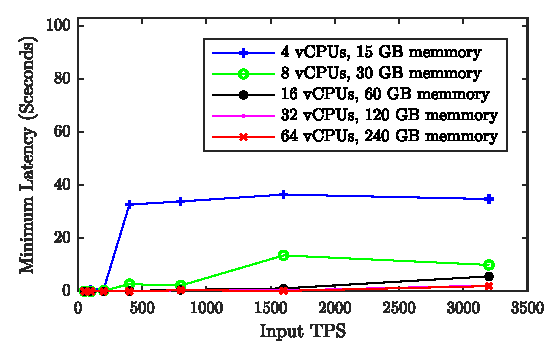
\includegraphics[width=\columnwidth]{figs/min.eps}%
\caption{Minimum Transaction Latency}%
\label{latency_min}%
\end{subfigure}\hfill%
\begin{subfigure}{0.99\columnwidth}
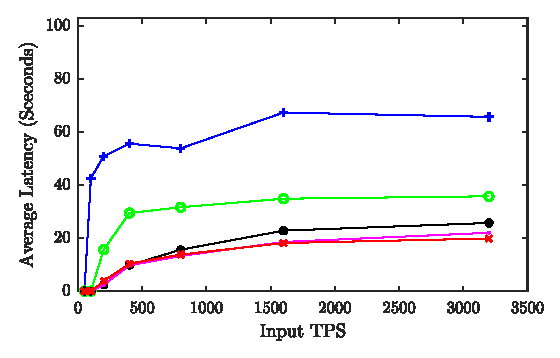
\includegraphics[width=\columnwidth]{figs/avg.eps}%
\caption{Average Transaction Latency}%
\label{latency_avg}%
\end{subfigure}\hfill%
\vspace{7mm}
\begin{subfigure}{0.99\columnwidth}
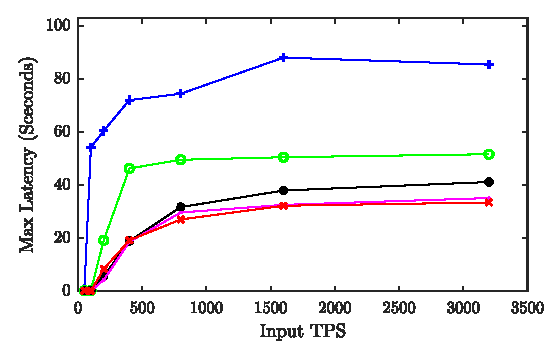
\includegraphics[width=\columnwidth]{figs/max.eps}%
\caption{Maximum Transaction Latency}%
\label{latency_max}%
\end{subfigure}\hfill%
\begin{subfigure}{0.99\columnwidth}
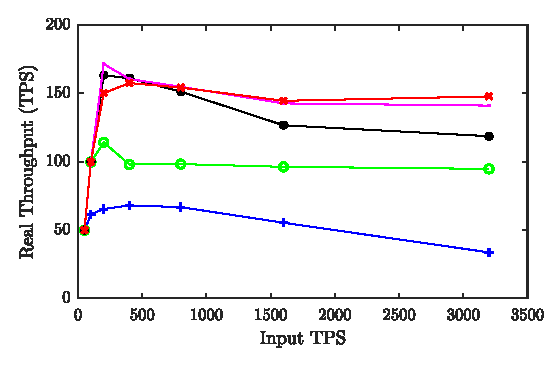
\includegraphics[width=\columnwidth]{figs/tps.eps}
\caption{Input vs. Real Transaction Throughput}
\label{fig:TPS}
\end{subfigure}\hfill%
\caption{Benchmark results on different virtual machine instances}
\label{latency}%
% \vspace{-9mm}
\end{figure*}

\section{Results}

The feasibility analysis and design of the blockchain application require comprehensive tests and performance measuring. In this section, we report the results of our experiments, using one of the most prominent blockchain frameworks. We will first introduce the experiment setup and then briefly analyze the results obtained.

\subsection{The Experiment Setup}
We run the benchmarks over an implementation of Hyperledger Fabric version 1.1 and using Hyperledger Caliper \cite{caliper}, which is a blockchain benchmark tool designed to enable performance measurements in different blockchain platforms including Hyperledger Fabric. The benchmarks provide results regarding the performance metrics mentioned in the previous section.

The network deployed for the experiment consists of 3 organizations, each operating one peer running inside a Docker container. We use the Fabric-CCP Node.js adaptor to communicate with the Fabric network. Each benchmark runs 5000 transactions with different transaction send rates (i.e., 50, 100, 200, 400, 800, 1600, 3200 TPS). The experiments are repeated on five different virtual machines hosted on Google Cloud platform (i.e., 64 vCPUs with 240 GB memory, 32 vCPUs with 120 GB memory, 16 vCPUs with 60 GB memory, 8 vCPUs with 30 GB memory and 4 vCPUs with 15 GB memory).

The benchmark uses transaction generating clients to generate tables of bids/asks representing the traders' supply and demand of resources. The transaction also hosts the logic of the auction mechanism which determines the final allocation of the resources and the price. In the next step, the endorsing peers endorse the transaction (i.e., the outcome of the auction) using the N-of-N endorsement policy meaning that all of the peers have to endorse the transactions in order for them to be validated. Finally, the orderer receives the endorsed transactions and orders them into a block to be written on the ledger.

The minimum, average, and maximum latency of the transactions are depicted in Fig. \ref{latency}. In Fig. \ref{latency_min}, the minimum latency experienced in the case of 4vCPU VM, illustrates a significant surge when the send rate goes beyond 200 TPS. The same pattern repeats in the average and maximum latency Fig. \ref{latency_avg} and Fig. \ref{latency_max} once the input load reaches the threshold of the processing capacity in 4vCPU VM.


%The initial smaller sudden surge (4vCPU plot) and then the return to lower latency could be explained by the fact that at this point,  Fabric is unable to process all of the transaction due to the overloading and is only able to process a quarter of the proposed transactions. As the send rate is increased to 200, the number of successful transaction decreases even further, and only 10\% of the transactions are successful. 
% \textcolor{red}{I removed the explanation of the initial surge as to me it's not explaining it.. unless you want to explain it further. Maybe if you introduce a graph with percentage of successful transactions, that would start making sense}. \textcolor{blue}{I added a table with percentages of failed transaction. It only fails in 4vCPU VM. See Table.\ref{failrate}}


On the other hand, the results for the 32vCPU and 64vCPU VMs indicate that the two-fold computing power increase does not affect the latency considerably as the Fabric reaches its logical performance limit. This is due to the sequential nature of the transaction endorsement and validation process.

The maximum latency experienced, shown in Fig. \ref{latency_max} indicates that in the case of the 4vCPU VM, the experienced maximum latency can reach as high as 88.12 seconds (average latency of 67.41 seconds) while achieving a throughput of 55.4 TPS. Using the 64vCPU VM, however, can perform with a maximum latency as small as 0.2 seconds (average latency of 0.07 seconds) with a throughput of 100 TPS.
The maximum latency is of great importance as it could be a determining factor in evaluating the feasibility of candidate blockchain use-cases. The maximum latency would determine whether the blockchain network can meet the latency requirements of the application. Furthermore, it will provide the information for hardware provisioning to host the blockchain network. 


Fig. \ref{fig:TPS} illustrates the performance of the blockchain application by comparing the input TPS (the transaction send rate) with the real transaction throughput achieved. The experiments are designed in an environment where the proposed transactions are generated by a built-in (local) load generation client to examine the VMs' capability not only for processing the transactions but also their performance for generating transaction proposals. A further study could assess the use of isolated and external load generation and investigate the behaviour of the VMs under equal pressure.

\begin{figure}
    \centering
    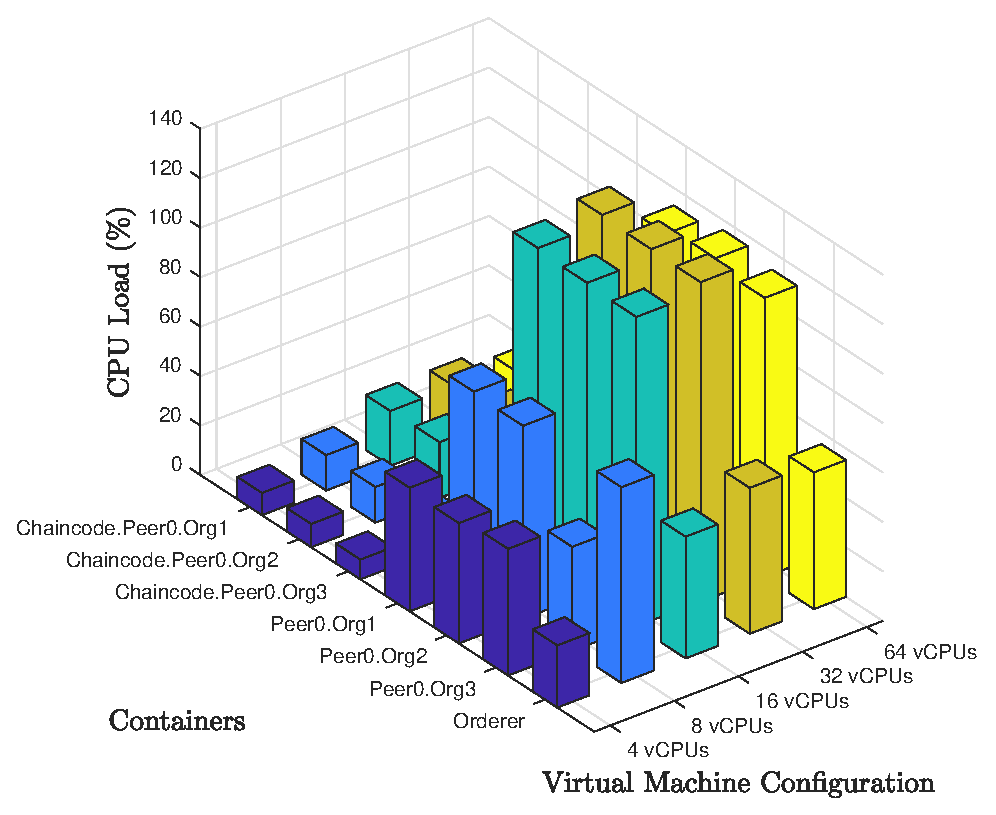
\includegraphics[width=0.49\textwidth]{figs/cpu.eps}
    \caption{CPU Performance of the Blockchain Application}
    \label{fig:cpu}
\end{figure}

The processing performance of the different components of the Fabric network is shown in Fig.  \ref{fig:cpu}. Each one of the components is hosted in a Docker container, as shown in the figure (i.e., Chaincode containers, peers, orderer, etc.). The CPU load is considerably lower in the less powerful VMs. This is due to the sequential nature of the transaction processing in Fabric blockchain. To elaborate, the execution, ordering and the verification of the block depend on the execution of the previous transactions. Therefore, since the less powerful VMs are not capable of processing with high throughput, this becomes a bottleneck and results in the under-utilization of the processing resources. 


Nonetheless, the performance of the Fabric heavily relies on the experimental setup and the configuration of the framework, network and the computing resources. For instance, the geographical distribution of the organizations and therefore, the peers could have huge effects on the performance. In addition, blockchain specific configuration such as block size (i.e., the number of transactions packed into a block) \cite{DBLP:journals/corr/abs-1805-11390} will affect the latency and throughput of the system. The white-paper \cite{hgperf} from the Hyperledger Performance and Scale Working Group \cite{pswg} provides an in-depth insight into the performance metrics and the factors associated with them.

The results from our experiments indicate best-case average latency of 70 milliseconds and best-case transaction throughput of 171 TPS. However, many studies claim that with precise design and implementation of the Hyperledger Fabric applications, it is possible to reach transaction throughputs as high as tens of thousands of transactions per second. For example, FastFabric \cite{fastFabric} is a project aiming to scale Hyperledger Fabric to support 20,000 transactions per second compared to the current supported throughput 3,000 TPS. This is done through architectural improvements to reduce computation and I/O overhead during transaction ordering and validation. FastFabrics's optimizations are fully plug-and-play and do not require any interface changes to the Hyperledger Fabric.



\section{Conclusions}
In this paper, we introduced a distributed approach to the bilateral trade markets for future telecommunications networks. We first described the research areas where bilateral trade markets are being adopted and the game-theoretic solutions for the allocation of commodities. Then we argued that the current trust on the central third-party brokers might not be sustainable as new network ownership models will provide market manipulation incentives for these brokers. As the main contribution of this paper, we discussed how blockchain technology, along with smart contracts, can help the bilateral trade markets to function in an untrusted environment. To examine the feasibility of our proposal, we implemented the proposed market model using an open source blockchain framework, Hyperledger Fabric. Finally, we reported the results of our experiments and analyzed how the proposed distributed market performs under different loads and also how these differences affect performance metrics such as latency and transaction throughput.
\section*{Acknowledgment}

Financial support from Science Foundation Ireland grants 14/IA/252 (O'SHARE) and 13/RC/2077 is gratefully acknowledged. This material is based upon work supported by Google Cloud.

\bibliographystyle{IEEEtran}
\bibliography{IEEEabrv,refs}



\begin{figure*}
% \vspace{-7mm}
\centering
\begin{subfigure}{0.99\columnwidth}
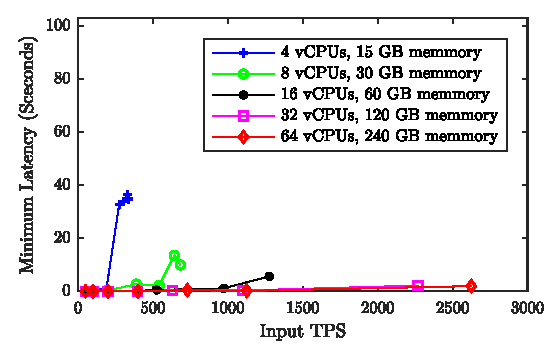
\includegraphics[width=\columnwidth]{figs/minLoad.eps}%
\caption{Minimum Transaction Latency}%
\label{latency_min}%
\end{subfigure}\hfill%
\begin{subfigure}{0.99\columnwidth}
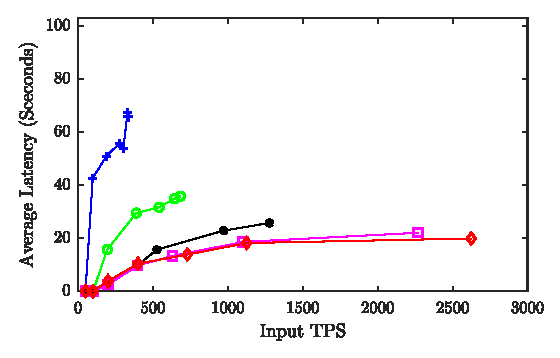
\includegraphics[width=\columnwidth]{figs/avgLoad.eps}%
\caption{Average Transaction Latency}%
\label{latency_avg}%
\end{subfigure}\hfill%
\vspace{7mm}
\begin{subfigure}{0.99\columnwidth}
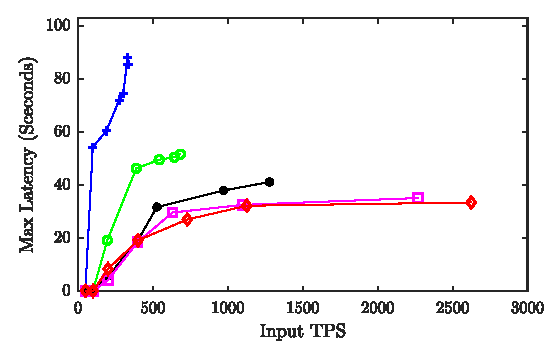
\includegraphics[width=\columnwidth]{figs/maxLoad.eps}%
\caption{Maximum Transaction Latency}%
\label{latency_max}%
\end{subfigure}\hfill%
\begin{subfigure}{0.99\columnwidth}
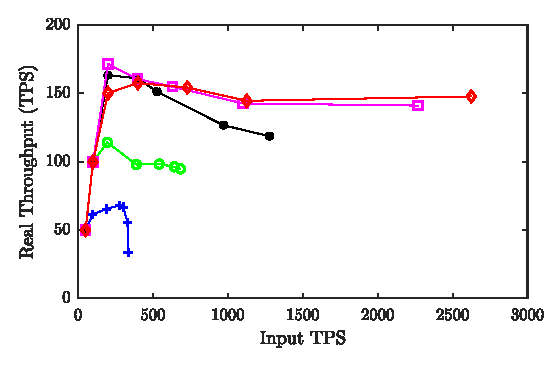
\includegraphics[width=\columnwidth]{figs/tpsLoad.eps}
\caption{Input vs. Real Transaction Throughput}
\label{fig:TPS}
\end{subfigure}\hfill%
\caption{Benchmark results on different virtual machine instances}
\label{latency}%
% \vspace{-9mm}
\end{figure*}



\begin{figure}
    \centering
    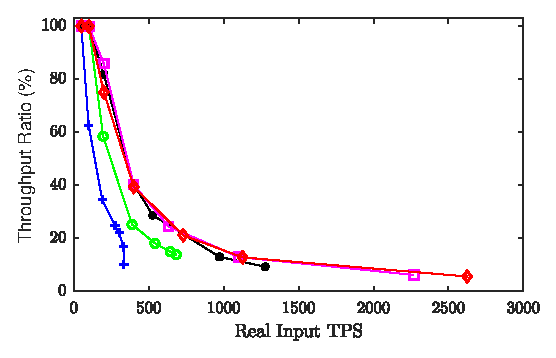
\includegraphics[width=0.49\textwidth]{figs/percentage.eps}
    \caption{Percentage of satisfied transactions out of submitted}
    \label{fig:cpu}
\end{figure}

\end{document}
